\subsection[]{Verifikation der Funktion eines phasenempfindlichen Gleichrichters}

Zur Verifikation der Funktionsweise eines phasenempfindlichen Gleichrichters werden insgesamt fünf verschiedene Phasen $\phi$ überprüft,
die in Abbildung \ref{fig:phasenunterschiede} einzusehen sind.

\begin{figure}%
    \begin{subfigure}{0.5\textwidth}%
    \centering%
    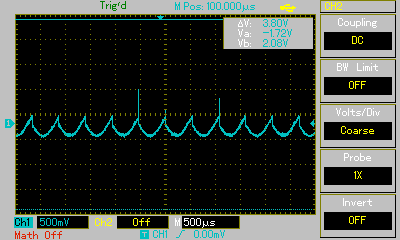
\includegraphics[width = 7.3cm]{./Oszilloskop Bilder/png/5.2/1 MAP002.png}%
    \caption{$\phi = \qty[]{0}{\degree}$}%
    \label{fig:phase1}%
    \end{subfigure}%
    %
    \hfill% Fills available space in the center -> space between figures
    \begin{subfigure}{0.5\textwidth}%
    \centering%
    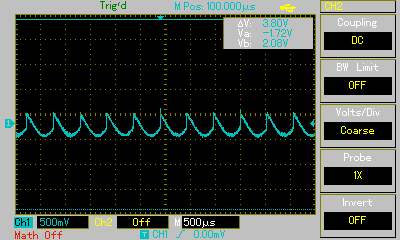
\includegraphics[width = 7.3cm]{./Oszilloskop Bilder/png/5.2/2 MAP003.png}%
    \caption{$\phi = \qty[]{45}{\degree}$}%
    \label{fig:phase2}%
    \end{subfigure}%
    %
    \hfill
    \begin{subfigure}{0.5\textwidth}%
    \centering%
    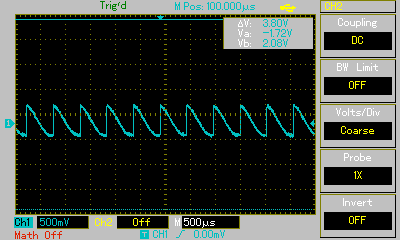
\includegraphics[width = 7.3cm]{./Oszilloskop Bilder/png/5.2/3 MAP004.png}%
    \caption{$\phi = \qty[]{90}{\degree}$}%
    \label{fig:phase3}%
    \end{subfigure}%
    %
    \hfill% Fills available space in the center -> space between figures
    \begin{subfigure}{0.5\textwidth}%
    \centering%
    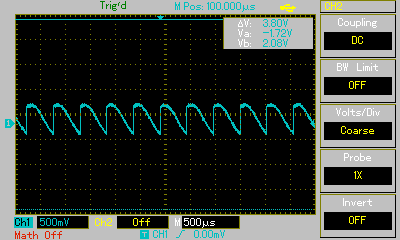
\includegraphics[width = 7.3cm]{./Oszilloskop Bilder/png/5.2/4 MAP005.png}%
    \caption{$\phi = \qty[]{135}{\degree}$}%
    \label{fig:phase4}%
    \end{subfigure}%
    %
    \hfill
    \begin{subfigure}{0.5\textwidth}%
    \centering%
    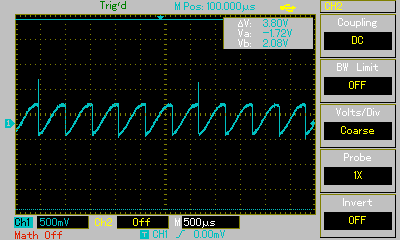
\includegraphics[width = 7.3cm]{./Oszilloskop Bilder/png/5.2/5 MAP006.png}%
    \caption{$\phi = \qty[]{180}{\degree}$}%
    \label{fig:phase5}%
    \end{subfigure}%
    %
    \caption{Spannungsverläufe für unterschiedliche Phasen}%
    \label{fig:phasenunterschiede}%
\end{figure}%
    

\begin{table}
    \centering
    \caption[]{Amplitude der Ausgangsspannung nach Integration}
    \label{tab:u_out_tp_ohne_noise}
    \sisetup{table-format=3.0}
    \begin{tabular}[]{S S}
        \toprule
        {$\phi / \unit[]{\degree}$} & {$U_\text{out} / \unit[]{\volt}$} \\
        \midrule
           0 &  \\
          45 &  \\
          90 &  \\
         135 &  \\
         180 &  \\
         225 &  \\
         270 &  \\
         315 &  \\
         300 &  \\
         330 &  \\
        \bottomrule
    \end{tabular}
\end{table}